% LNCS paper, based on samplepaper.tex
\documentclass[runningheads]{llncs}

\usepackage[T1]{fontenc}
\usepackage{graphicx}
\usepackage{booktabs}
\usepackage{tabularx}
\usepackage{array}
\usepackage{amsmath}
\usepackage{xcolor}
\newcommand{\TODO}[1]{\textcolor{red}{\textbf{[#1]}}}
\usepackage[section]{placeins}

\newif\ifanonymous
%\anonymoustrue      % wersja do double blind review
\anonymousfalse   % wersja camera-ready


\begin{document}

\title{Prediction or Revaluation? Phase- and Space-Aware VAEP for Women's Football}

\titlerunning{Phase-Space VAEP for Women's Football}
\ifanonymous
  \author{Anonymous Author(s)}
  \authorrunning{Anonymous Author(s)}
  \institute{Paper under double-blind review}
\else
\author{
Tomasz Piłka\inst{1}\orcidID{0000-0003-1206-2076} \and
Kaj Skubiszak\inst{2}\orcidID{0009-0003-9004-4620} \and 
Piotr Andrzejewski\inst{3}\orcidID{0009-0001-3721-6046} \and 
Patryk Żyliński\inst{4}\orcidID{0009-0002-2119-5292}
}

\authorrunning{T. Piłka et al.}

\institute{Faculty of Mathematics and Computer Science, \\Adam Mickiewicz University in Pozna\'n, Poland \\
\email{tomasz.pilka@amu.edu.pl} \\
\email{\{kajsku, pioand6, patzyl\}@st.amu.edu.pl}}
\fi 

\maketitle
\begin{abstract}
Event-based action valuation models, such as VAEP, assign value to on-ball actions based on their type, outcome, location, and recent context, but they do not encode the off-ball spatial configuration in which the action is performed. This limitation is particularly relevant in women's football, where public spatial data remains scarce. We study whether two interpretable context layers, rule-based tactical phase labels and geometric features from StatsBomb 360 freeze frames, affect VAEP-style action valuation in a men-to-women source-target learning setting.

We compare four variants in a $2 \times 2$ design over the two context layers: Event-VAEP, Phase-VAEP, Event-Space VAEP and Phase-Space VAEP. The models are evaluated on a held-out women's tournament in terms of discrimination, calibration, source-target training strategy and player valuation behaviour, with paired match-level bootstrap intervals throughout. Tactical phase information improves estimation of conceding risk, by $+0.006$ ROC-AUC averaged over ten seeds, while its effect on the scoring head is negligible. Freeze-frame spatial features do not improve aggregate discrimination and degrade it when combined with phase, the two layers acting as substitutes rather than complements; they nonetheless reorder the player ranking substantially, from $\rho = 0.98$ to $\rho = 0.82$ against the event-only baseline. We characterise this redistribution without treating it as a correction, and a stratified analysis does not identify the situations responsible. We further show that the spatial features are recoverable from event data well enough that a model built on predicted rather than observed freeze frames performs equally well, and that source-domain similarity is governed more by competition type than by gender. The results show that contextual action valuation should be assessed not only by predictive metrics but also by how value is allocated --- and that both comparisons demand a single action set and explicit accounting for training-time as well as evaluation-time variability.

\keywords{action valuation \and VAEP \and women's football \and StatsBomb 360 \and spatial features \and transfer learning \and football analytics}
\end{abstract}


\section{Introduction}

Football action valuation aims to assign credit to individual on-ball actions by estimating how much they change a team's probability of scoring and conceding. Valuing Actions by Estimating Probabilities (VAEP) is one of the most widely used frameworks for this task because it values all on-ball actions, not just shots \cite{decroos2019actions}. However, classical VAEP is primarily event-based: it observes action type, result, location, body part, time, score state and a short history of previous actions, but not the spatial configuration of off-ball players around the action.

This creates two distinct limitations, which motivate two different context layers.

The first is spatial. Two actions with the same event description may differ substantially in tactical difficulty. A pass or take-on performed under pressure, through a compact defensive block, is not equivalent to the same action performed in open space. Event-only valuation cannot distinguish these cases and may therefore assign value incorrectly when pressure, congestion or defensive structure matter more than ball trajectory alone.

The second concerns the possession regime rather than the local geometry. Canonical VAEP conditions on a fixed-length history of three preceding actions, which represents the recent past but not whether a possession is settled or has just changed hands. Two own-third passes can agree in action type, body part, start and end coordinates, score state, and all three preceding actions, yet still carry very different risks depending on whether they occur during a controlled build-up or seconds after a turnover against a team pressing forward. Because the phase governs how severely a turnover is punished rather than how likely a goal is at the other end, this omission should bear primarily on the conceding side of the valuation -- a prediction we test directly in Section~\ref{sec:ablation}.

The limitation is especially relevant in women's football. Event data for women's competitions is increasingly available, but public spatial data remains much more limited than in men's football. StatsBomb 360 freeze frames provide an intermediate form of spatial context: they record the visible players at the moment of each event, but not their continuous trajectories \cite{statsbomb2021freezeframe}. This makes them suitable for compact, interpretable features that describe local pressure, support, defensive density, and zone occupation.

We study whether such contextual changes affect VAEP-style action valuation in women's football. Specifically, we add two interpretable layers to an event-only VAEP baseline: rule-based tactical phase labels and geometric spatial features extracted from StatsBomb 360 freeze frames. We evaluate the resulting nested models--Event-VAEP, Phase-VAEP and Phase-Space VAEP--in a controlled ablation study and in a men-to-women source-target training setting.

The paper makes three contributions. First, we propose a compact, interpretable extension of VAEP that combines tactical phase annotation with freeze-frame spatial features, and evaluate the two layers in a full $2 \times 2$ design that separates their main effects from their interaction. Second, we compare women-only training, men-only zero-shot transfer, sequential fine-tuning and pooled source-target training for a data-scarce target domain, using size-matched and domain-balanced comparisons to distinguish the value of additional data from the value of cross-domain data. Third, we separate predictive performance from valuation behaviour: phase context improves estimation of conceding risk, whereas spatial context leaves aggregate prediction broadly unchanged while substantially reallocating value across players, positions and tactical situations. All comparisons are reported with paired match-level bootstrap intervals, and we characterise the reallocation without treating it as a correction.

\section{Related Work}

\subsection{Action Valuation in Football}

Football action valuation addresses the problem of assigning credit to individual on-ball actions in a low-scoring and highly contextual sport. Traditional player
evaluation based on goals, assists, shots or expected goals captures only a small fraction of the actions that shape possession. More general possession-value and
action-value models instead represent football as a sequence of game states and estimate how actions change the value of the resulting state \cite{decroos2019actions,liu2020deep}.

The most directly related framework is Valuing Actions by Estimating Probabilities (VAEP), introduced by Decroos et al. \cite{decroos2019actions}. VAEP represents matches as sequences of standardised on-ball actions and estimates two probabilities for each game state: scoring and conceding within a fixed action horizon. This makes it possible to value all on-ball actions, not only shots or passes, and to separate offensive and defensive contributions. A parallel line of work values specific action types, most directly the pass-valuation framework of Bransen et al.~\cite{bransen2019passes}, developed alongside rather than after VAEP. Later work has extended action valuation to additional learning paradigms, including deep reinforcement learning approaches to soccer action value~\cite{liu2020deep}. However, these approaches remain primarily grounded in event streams and therefore do not directly observe the off-ball spatial configuration around the action.

\subsection{Spatial Context and Freeze-Frame Data}

A separate line of work shows that spatial context is central to football analytics. Dominant-region, pitch-control and expected-possession-value models use player locations to evaluate space occupation, receiving opportunities and the risk or reward of actions \cite{taki2000dominant,spearman2018beyond,power2017passes,fernandez2018wide,fernandez2021framework}. Related work has also explored visually interpretable spatial representations of football actions, for example by learning pitch-level probability surfaces for passing
options and action outcomes \cite{fernandez2021soccermap}.

The most closely related freeze-frame valuation model is the VAEP360 variant used in Un-XPass~\cite{robberechts2023unxpass}, from which our approach differs on three axes. In terms of objectives, VAEP360 supports the evaluation of passing decisions and player creativity, whereas we value the complete on-ball action stream, including carries, take-ons, and defensive actions. In representation, VAEP360 consumes the freeze frame via learned surface-based spatial representations, whereas we use a compact set of handcrafted geometric features chosen for interpretability and robustness under partial broadcast visibility. In the data regime, our target domain is small and distributionally distinct from the source, which is what motivates a low-capacity encoding rather than a learned one. The two routes are complementary rather than competing. The phase layer we propose is a property of the game state rather than of the spatial encoder, and could therefore be supplied to a learned model such as VAEP360 without modification; a direct empirical comparison under our source-target protocol is left to future work.

Most of these models assume access to continuous tracking data for all players and the ball. Such data is rarely public and remains especially limited in women's football. StatsBomb 360 freeze frames provide an intermediate form of spatial context: they record the visible players at the moment of each event, but not their trajectories \cite{statsbomb2021freezeframe}. This enables lightweight spatial features such as nearest-opponent distance,  defensive density and opponents between the ball and the goal. Recent work has used the same freeze-frame context to evaluate passing decisions and player creativity \cite{robberechts2023unxpass}. Our work follows this interpretable freeze-frame route, but integrates such features into VAEP-style action valuation rather than pass-choice evaluation.

\subsection{Source-Target Learning for Data-Scarce Sports Analytics}

A further relevant line of work concerns transfer learning and domain adaptation. Standard supervised learning assumes that training and test data come from the same distribution, whereas transfer learning uses information from a source domain to improve learning in a related target domain \cite{pan2010survey}. Domain adaptation theory further relates target-domain error to source-domain error and to the divergence between domains \cite{bendavid2010theory}.

This setting is directly relevant to women's football analytics. Public event data for women's competitions is increasingly available, but public spatial data remains much more limited than in men's football. Training a spatially aware valuation model only on a small women's 360 corpus risks overfitting, while training only on men's football risks domain shift. We therefore treat men's 360 football as a data-rich source domain and women's football as a data-scarce target domain, comparing women-only training, zero-shot transfer, sequential fine-tuning and pooled source-target training. To our knowledge, the combination of VAEP-style action valuation, StatsBomb 360 freeze-frame features and men-to-women source-target learning remains underexplored.

\section{Data, Models and Training}

\subsection{Data and Splits}

The dataset is Hudl StatsBomb's public open-data release, accessed through the official open-data repository \cite{statsbomb2026opendata}. Event data describes each on-ball action --- pass, dribble, shot, tackle, clearance, set-piece restart --- with type, result, body part, location, and a structured timestamp. StatsBomb 360 augments these events with a freeze frame: at the instant of each event, the two-dimensional pitch positions of every player visible in the broadcast view, each labelled as actor, teammate, or opponent, and separately as a goalkeeper or outfield player~\cite{statsbomb2021freezeframe}. A visible-area polygon delimits the region the broadcast camera captured. Freeze frames are not continuous tracking: positions are sampled only at event moments and only within the camera's field of view, and some players are systematically not recorded. The freeze-frame features described below are designed to be robust to this partial visibility. Because coverage is itself systematically related to pitch position, we additionally record three coverage measures for each event -- the area of the visible-area polygon, the number of visible players, and the actor's distance to the polygon boundary -- and use them in Section~\ref{sec:visibility} to test whether the valuation effects we report track defensive structure or broadcast framing.

\subsection{Train, Adaptation, and Evaluation Splits}
We organise the StatsBomb data into four corpora with distinct experimental roles (Table~\ref{tab:corpora}). Men's 360 data forms the source domain, women's 360 data provides target-domain adaptation data, and UEFA Women's Euro 2025 is reserved as a held-out evaluation tournament. A separate women's event-only corpus is included only to show the asymmetry between the broad availability of event data and the much narrower availability of freeze-frame spatial data.

\begin{table}[!htbp]
\centering
\scriptsize
\caption{StatsBomb corpora and experimental roles. The evaluation corpus is held out from all training and model selection.}
\label{tab:corpora}
\begin{tabular}{@{}ll l r r r@{}}
\toprule
\textbf{Corpus} & \textbf{Domain} & \textbf{Role} &
\textbf{Matches} & \textbf{Events} & \textbf{360 frames} \\
\midrule
Men's 360 source
& Men
& Source training
& 200
& 752{,}967
& 652{,}881 \\

Women's 360 adaptation
& Women
& Target training / calibration
& 95
& 331{,}303
& 284{,}305 \\

Women's 360 evaluation
& Women
& Held-out test
& 31
& 105{,}611
& 90{,}722 \\

Women's event-only context
& Women
& Descriptive context only
& 414
& 1{,}386{,}529
& --- \\
\bottomrule
\end{tabular}
\end{table}

The men's 360 source corpus includes FIFA World Cup 2022, UEFA Euro 2020, UEFA Euro 2024, and Bundesliga 2023/24. The three international tournaments match the target domain's competition type. Bundesliga 2023/24 was included because it is the largest men's 360 corpus in the public release, and excluding it would have substantially reduced the source domain; this is a data-availability decision rather than a claim that club football is the more similar source. Since competition type may matter as much as gender for domain similarity, we treat the composition as a variable rather than a fixed choice: Section~\ref{sec:transfer} reports transfer from the international and club subsets separately under a size-matched protocol, together with pairwise domain-divergence estimates. The women's 360 adaptation corpus includes FIFA Women's World Cup 2023 and UEFA Women's Euro 2022, while UEFA Women's Euro 2025 is reserved as the held-out evaluation tournament. The additional event-only corpus covers FIFA Women's World Cup 2019, NWSL 2018, and three FA Women's Super League seasons.

The corpus counts in Table~\ref{tab:corpora} refer to raw StatsBomb events, whereas the evaluation counts reported below refer to the SPADL-converted action stream after filtering to VAEP-eligible actions.

\subsection{Model Variants}

\paragraph{\textbf{Event-VAEP.}}
Following Decroos et al. \cite{decroos2019actions}, Event-VAEP (E-VAEP) estimates two probabilities for each game state $s_i$ reached after action $a_i$: the probability that the acting team scores within the next $k = 10$ actions, $P_{\text{score}}(s_i)$, and the probability that it concedes within the same window, $P_{\text{concede}}(s_i)$. The value of action $a_i$ is the change these probabilities undergo across it:
\[
V(a_i) = \big[\, P_{\text{score}}(s_i) - P_{\text{score}}(s_{i-1}) \,\big] - \big[\, P_{\text{concede}}(s_i) - P_{\text{concede}}(s_{i-1}) \,\big].
\]
Each probability is estimated by a separate binary classifier trained on the SPADL-converted action stream. E-VAEP uses the canonical VAEP feature set: action type, result, body part, start and end coordinates, distance and angle to goal, elapsed time and time-delta, score state, and the same fields for the three preceding actions. It carries no information about any player other than the actor.

\paragraph{\textbf{Phase-VAEP.}}

Phase-VAEP (P-VAEP) extends E-VAEP with a six-class tactical phase label: \emph{build-up}, \emph{progression}, \emph{final-third creation}, \emph{transition attack}, \emph{defensive transition}, and \emph{set piece}. We assign labels by an explicit set of rules for interpretability. A zone default uses the SPADL coordinates of the action: actions in the attacking third are final-third creation, in the own third build-up, and otherwise progression. Three context-sensitive rules override the zone default in increasing priority. A defensive action --- tackle, interception, clearance, block or foul --- played in the own third immediately after a possession change is a defensive transition. An action within five seconds of a possession that began with a recovery or a counter-attack is a transition attack. Any action that is itself a restart, or the first action of a possession that began from one, is a set piece. The one-hot phase label and its interactions with action type are added to the feature set. Crossing all six phases with all 21 SPADL action types would give 126 largely empty indicators, so action types are first grouped into seven families --- pass, carry, take-on, shot, defensive, goalkeeper and restart --- yielding 42 interaction indicators, of which 11 are structurally empty because the combination cannot occur.

\paragraph{\textbf{Event-Space VAEP.}}

Event-Space VAEP (ES-VAEP) adds the spatial features described below to E-VAEP without the phase layer. It completes the $2 \times 2$ design over the two context layers, which is what allows the main effect of each layer to be estimated separately from their interaction: the phase effect is identified by both $(\mathrm{P} - \mathrm{E})$ and $(\mathrm{PS} - \mathrm{ES})$, the space effect by both $(\mathrm{ES} - \mathrm{E})$ and $(\mathrm{PS} - \mathrm{P})$, and the interaction by the difference between the two estimates of either.

\paragraph{\textbf{Phase-Space VAEP.}}
\label{sec:spatial}

Phase-Space VAEP (PS-VAEP) extends P-VAEP with seventeen geometric features computed from each StatsBomb 360 freeze frame. Coordinates are normalised so that the acting team attacks from left to right, and distances are computed on a $105 \times 68$ m pitch. The features capture four interpretable aspects of the visible spatial context: pressure and support, measured by nearest-opponent and nearest-teammate distances; defensive density, measured by the number of visible opponents within 5, 10 and 15 m of the ball and in a forward cone; defensive structure, measured by opponents ahead of the ball and inside the ball-goal corridor; and zone context, including central, half-space, wide, box, box-entry and final-third-entry indicators. These features are deliberately compact and use only the players visible in the freeze frame \cite{statsbomb2021freezeframe}.


\subsection{Training and Evaluation Protocol}

All variants share the same classifier. We use LightGBM~\cite{ke2017lightgbm} because the feature set is tabular, low-dimensional and mixes categorical with continuous variables; because both target classes are rare; because the target corpus is small; and because gradient-boosted trees are the standard learner in the VAEP literature and in the reference implementation, which keeps our results comparable with prior work. Hyperparameters (63 leaves, learning rate $0.05$, up to 1500 boosting rounds with early stopping after 50 rounds without validation-loss improvement) are taken from that reference configuration and held fixed across all variants and strategies rather than tuned per variant, so that differences between variants are attributable to the feature set alone. Because several of those differences are small, we report their sensitivity to this choice in Section~\ref{sec:sensitivity}: ten random seeds per model--strategy cell, a small grid over the number of leaves, learning rate and feature fraction, and logistic-regression and XGBoost~\cite{chen2016xgboost} baselines. Seed variation turns out to be large relative to the differences between variants, so we report every headline effect as a mean over ten seeds rather than from a single run. The two heads --- scoring and conceding --- are trained as independent binary classifiers. Splits are at the match level to prevent within-match leakage: within the training corpus, 15\% of matches are reserved as a validation fold for early stopping; the test set is the entire UEFA Women's Euro 2025 tournament, disjoint from all training data. All variants are trained on identical corpora for each strategy and differ only in their input feature sets.


\subsection{Source-Target Training Strategies}

Given the limited availability of women's 360 data, we examine how to combine men's and women's training corpora. We evaluate four strategies. \emph{Women-only} training uses only the women's 360 adaptation corpus, as a control. \emph{Men-only zero-shot} transfer applies a model trained purely on men's data to women's actions without further adaptation. \emph{Fine-tuned} pre-trains on men's data and continues boosting on women's data at a reduced learning rate. \emph{Pooled} training trains a single model on the union of men's and women's data. We additionally test post-hoc isotonic recalibration on a held-out women's calibration fold. Because pooled training uses more data than either single-domain strategy, a pooled advantage alone cannot distinguish cross-domain complementarity from a sample-size effect. We therefore add three controls: a size-matched comparison in which the men's corpus is subsampled to the 95 matches of the women's adaptation corpus; a domain-balanced pooled variant with equal match counts per domain; and learning curves in the number of training matches, computed separately for each source composition. We also report the effect of the post-hoc isotonic recalibration on the probability metrics.



\subsection{Evaluation Metrics}

We report two families of metrics. Discrimination is measured by ROC-AUC and average precision (AP). ROC-AUC weights positives and negatives symmetrically; AP is more sensitive to the rare positive class, which is appropriate given baseline positive rates of approximately 1.5\% for scoring and 0.34\% for conceding. Probability quality is measured by Brier score, log loss, and Expected Calibration Error (ECE)~\cite{guo2017calibration}. Because the conceding positive rate is approximately $0.34\%$, equal-width binning places nearly all actions in the lowest bin and is close to uninformative at this scale. We therefore report ECE over equal-frequency bins with a sensitivity check over the number of bins, and support the calibration claims with reliability diagrams on a logarithmic probability axis and with a decomposition of the Brier score into reliability and resolution components, which separates loss of calibration from loss of resolution. Player-valuation effects are reported through Spearman rank correlations between model rankings.

Because PS-VAEP is defined only for actions with freeze-frame coverage (51{,}172 of 60{,}370 evaluation actions), the ablation comparison must be matched accordingly. We therefore report all metrics in this paper -- both the ablation of Table~\ref{tab:ablation} and the source-target comparison of Table~\ref{tab:transfer} -- on the identical 51{,}172-action 360 subset. Reporting E-VAEP and P-VAEP on the full 60{,}370-action set, while restricting PS-VAEP to its 51{,}172, would compare different action sets and systematically advantage PS-VAEP on score-head metrics, because the actions without a freeze frame are, by definition, harder broadcast-gap moments.

\paragraph{\textbf{Uncertainty.}}
All reported differences carry paired match-level bootstrap intervals~\cite{efron1993bootstrap}. We resample the 31 evaluation matches with replacement ($B = 1000$) and recompute every metric for every variant on each resample. Because actions within a match are correlated, the match rather than the action is the resampling unit throughout, which corresponds to a cluster bootstrap~\cite{field2007bootstrapping}. Because all variants are evaluated on the identical action set, we form differences within each replicate and report percentile intervals for the difference rather than independent intervals per model, which is both the quantity our claims concern and a considerably tighter estimate. For the player analysis, the resampling unit is likewise the match: within each replicate we recompute per-player minutes and VAEP per 90 from the resampled matches before recomputing rank correlations and individual rank changes, rather than treating the 117 players as independent observations.

The bootstrap captures uncertainty from the evaluation sample but not from training. Because the training corpus is small and the positive classes rare, the train/validation split and the learner's own randomisation are a second, independent source of variation. We therefore repeat every headline comparison across ten seeds and report the paired difference averaged over them. The two sources are of comparable magnitude here, and reporting only one would understate the uncertainty substantially; Section~\ref{sec:sensitivity} shows that a single-seed estimate of the phase effect can exceed the ten-seed mean by a factor of four.

\section{Results}

\subsection{Transfer Learning}
\label{sec:transfer}

Table~\ref{tab:transfer} reports conceding-head ROC-AUC for the four source-target training strategies. Women-only training is weakest for every variant, indicating that the available women's 360 corpus is insufficient in isolation, and pooled source-target training is best for every variant. Sequential fine-tuning does not improve on zero-shot transfer, suggesting that continued boosting on the small target corpus adds less than joint training does.

\begin{table}[tbp]
\footnotesize
\centering
\caption{Conceding-head ROC-AUC by source-target training strategy. Best value per column in bold. All variants are evaluated on the identical 51{,}172-action 360 subset.}
\label{tab:transfer}
\begin{tabular}{lrrrr}
\toprule
\textbf{Strategy} & \textbf{E-VAEP} & \textbf{P-VAEP} & \textbf{ES-VAEP} & \textbf{PS-VAEP} \\
\midrule
Women-only (control) & 0.811 & 0.810 & 0.810 & 0.791 \\
Men-only (zero-shot) & 0.834 & 0.823 & 0.837 & 0.842 \\
Fine-tuned & 0.831 & 0.819 & 0.825 & 0.835 \\
\textbf{Pooled} & \textbf{0.837} & \textbf{0.865} & \textbf{0.840} & \textbf{0.849} \\
\bottomrule
\end{tabular}
\end{table}

The ranking among strategies is confounded, however, because pooled training also sees more data than either single-domain strategy. We therefore repeat the comparison with the men's corpus subsampled to the 95 matches of the women's adaptation corpus (Table~\ref{tab:sizematched}). At equal size the two single-domain strategies are indistinguishable --- men-only $0.822$ against women-only $0.821$ --- and performance tracks the number of training matches rather than their provenance. The conclusion the data support is therefore that additional 360 data helps regardless of whether it comes from men's or women's football, not that cross-domain training carries complementary information. For a data-scarce target domain this is the more useful finding of the two, since it means any available 360 corpus is worth adding.

\begin{table}[tbp]
\footnotesize
\centering
\caption{Size-matched source-target comparison for PS-VAEP, mean over five seeds. Performance tracks the number of training matches, not the domain they come from.}
\label{tab:sizematched}
\begin{tabular}{lrrr}
\toprule
\textbf{Strategy} & \textbf{Train matches} & \textbf{Conceding ROC-AUC} & \textbf{SD} \\
\midrule
Pooled, full & 295 & 0.854 & 0.006 \\
Men-only, full & 200 & 0.844 & 0.010 \\
Pooled, size-matched & 190 & 0.842 & 0.009 \\
Men-only, size-matched & 95 & 0.822 & 0.015 \\
Women-only & 95 & 0.821 & 0.009 \\
\bottomrule
\end{tabular}
\end{table}

The composition of the men's source also matters, and not in the direction gender alone would predict. Estimating a proxy $\mathcal{A}$-distance with a domain classifier trained to separate action feature vectors, men's international football sits at $0.713$ from the women's target while the men's club corpus sits at $0.955$, with the two men's subsets only $0.214$ apart. Size-matched transfer agrees: from 34 matches, an international source reaches $0.755$ and a club source $0.717$. Competition type is therefore the more important axis of similarity here, and Bundesliga is the more distant source despite matching the rest of the men's corpus on gender.

\subsection{Ablation: Event, Phase, and Space}
\label{sec:ablation}

Table~\ref{tab:ablation} shows the matched ablation on the identical 51,172-action 360 subset. Adding tactical phase information improves the conceding head, and this is the only improvement anywhere in the ablation whose bootstrap interval excludes zero. Averaged over ten seeds the paired effect is $+0.006$ (95\% CI $[+0.001, +0.011]$, positive in 8 of 10 seeds); the single-seed value in Table~\ref{tab:ablation} is $+0.027$, which sits at the extreme of the seed distribution. We report the seed-averaged figure as the effect and treat the tabulated run as one draw from it. The scoring head is unaffected, as the motivation in Section~1 predicts: phase governs how severely a turnover is punished, not how likely a goal is at the other end.

Adding spatial features on top of phase does not produce a comparable gain; it produces a loss. PS-VAEP is below P-VAEP on both heads and on conceding AP ($0.156$ against $0.178$), and the $2 \times 2$ design shows why this is not simply a failure of the spatial layer. The phase effect is $+0.027$ without space but only $+0.010$ once space is present, while the space effect is $+0.003$ without phase and $-0.015$ with it, giving an interaction of $-0.018$. The two layers are substitutes rather than complements: they encode overlapping information about how exposed a state is, and supplying both leaves the learner with redundant, noisier evidence than either alone. Neither main effect nor the interaction is individually separated from zero at $n = 31$ matches, so we present this as the pattern the design reveals rather than as three estimated quantities.


\begin{table}[!tbph]
\footnotesize
\centering
\caption{Matched ablation on the 51,172-action UEFA Women's Euro 2025 360 subset. Higher is better for ROC-AUC and AP; lower is better for log loss and ECE. All variants are evaluated on the identical 51{,}172-action 360 subset.}
\label{tab:ablation}
\begin{tabular}{lrrrr}
\toprule
& \textbf{E-VAEP} & \textbf{P-VAEP} & \textbf{ES-VAEP} & \textbf{PS-VAEP} \\
& (event) & (+ phase) & (+ space) & (+ both) \\
\midrule
Scoring ROC-AUC & 0.825 & 0.827 & 0.823 & 0.823 \\
Scoring AP & 0.291 & 0.293 & 0.292 & 0.288 \\
Scoring log loss & 0.0628 & 0.0626 & 0.0627 & 0.0629 \\
Scoring ECE ($10^{-3}$) & 3.8 & 3.8 & 3.7 & 3.9 \\
\midrule
Conceding ROC-AUC & 0.837 & \textbf{0.865} & 0.840 & 0.849 \\
Conceding AP & 0.171 & 0.178 & 0.167 & 0.156 \\
Conceding log loss & 0.0182 & 0.0178 & 0.0183 & 0.0182 \\
Conceding ECE ($10^{-3}$) & 1.4 & 1.2 & 1.1 & 1.1 \\
\bottomrule
\end{tabular}

\vspace{0.5em}
{\footnotesize
Bold marks the only difference whose paired match-level bootstrap interval excludes zero: P-VAEP over E-VAEP on conceding ROC-AUC, $+0.027$ (CI $[+0.013, +0.046]$) for this run, $+0.006$ (CI $[+0.001, +0.011]$) averaged over ten seeds. No calibration difference is robust under either equal-width or equal-frequency binning, so we make no calibration claim.
}
\end{table}

\subsection{Where the Added Context Matters}
\label{sec:where}

To locate the effect of the spatial layer we decompose the per-action change $\Delta = V_{\mathrm{PS}}(a) - V_{\mathrm{P}}(a)$ across defensive density, distance to the nearest opponent, pitch zone, action type and outcome, reporting the share of actions and the mean change with match-level bootstrap intervals in each stratum.

The result is negative, and we report it as such. No stratum shows a robustly positive mean change. Actions with three or more visible opponents within 5~m --- the stratum a congestion account predicts --- shift by $+0.0010$ with an interval of $[-0.0003, +0.0023]$ that includes zero. Distance to the nearest opponent produces no gradient at all ($-0.0018$, $-0.0017$, $-0.0012$ and $+0.0010$ across the density levels; $-0.0015$ to $-0.0013$ across distance bands), and pitch zone produces none either. By action type, the largest shifts fall on throw-ins and goalkeeper claims rather than on open-play progression.

We therefore do not claim a mechanism. The spatial layer demonstrably reallocates value, as Section~\ref{sec:players} shows, but the stratification does not identify the situations responsible. An earlier version of this analysis, run on models trained without the phase interactions, did find a robustly positive congestion stratum; that it did not survive retraining is itself a caution against reading mechanism into a redistribution of this size.

\subsection{Feature Groups and Event-Data Approximation}
\label{sec:groups}

Grouping the seventeen spatial features into pressure and support, defensive density, defensive structure and zone context, we compare add-one-group-in and leave-one-group-out variants against the event baseline, all trained on the freeze-frame subset so that the variants are mutually comparable. Two results stand out. Removing the defensive-density group \emph{improves} both conceding ROC-AUC ($0.860$ against $0.853$ with all groups) and conceding AP ($0.194$ against $0.159$), and removing defensive structure also helps; only zone context is clearly load-bearing, its removal costing $0.008$ ROC-AUC and $0.020$ AP. Grouped SHAP attributions rank pressure and support highest among the spatial groups, ahead of the phase layer, which illustrates that attribution measures how heavily a model leans on a feature and not whether leaning on it helps.

The more consequential question is whether the spatial features are available at all without 360 coverage. We fit a model predicting each spatial feature from event features alone, then rebuild the valuation model on the predicted values. The zone indicators are recovered perfectly, which is expected rather than informative --- they are deterministic functions of the action coordinates, and those coordinates are event features. The density and structure counts are recovered with $r^2$ between $0.39$ and $0.70$. Rebuilt on these predictions, \emph{Pseudo-Space VAEP} matches the model built on observed freeze frames and slightly exceeds it (conceding ROC-AUC $0.858$ against $0.853$; AP $0.161$ against $0.159$).

The spatial layer therefore contributes little that event data does not already imply, which is consistent with its absence of predictive benefit throughout this study. Practically, it means the approach transfers to competitions without freeze-frame coverage --- a useful property given how much more widely event data is available for women's football than 360 data.

\subsection{Freeze-Frame Visibility Controls}
\label{sec:visibility}

Freeze frames record only the players the broadcast camera captured, and coverage varies systematically with pitch position, so a positional redistribution could in principle reflect camera framing rather than defensive structure. Using the coverage measures of Section~3.1, the visible-area polygon covers a mean of $24\%$ of the pitch and the actor sits a median $6.7$~m from its boundary. Coverage does vary by zone in the direction the concern anticipates: a mean of $14.4$ visible players in the middle third against $12.2$ in the penalty area.

The association with the revaluation is nonetheless negligible. The Spearman correlation between the number of visible players and $\Delta$ is $0.020$ across the evaluation set and $0.065$ within the penalty area, the zone where the confound would bite hardest, and restricting to the better-covered half of actions or to actions at least 10~m inside the polygon boundary does not materially change the picture. Partial visibility bounds what the spatial features can encode, but it does not explain the redistribution we report.

\subsection{Sensitivity to Modelling Choices}
\label{sec:sensitivity}

Because several differences in Table~\ref{tab:ablation} are small, we quantify how much of that variation arbitrary choices could produce. Across ten seeds --- varying both the train/validation split and the learner's randomisation --- conceding ROC-AUC has a standard deviation of $0.006$ for E-VAEP and $0.009$ for P-VAEP, with ranges spanning $0.02$. Seed variation is therefore of the same order as the differences the ablation is asked to resolve, which is why we report the phase effect as a ten-seed mean.

Over a grid of $18$ hyperparameter settings (leaves $\in \{31, 63, 127\}$, learning rate $\in \{0.03, 0.05, 0.1\}$, feature fraction $\in \{0.6, 0.8\}$) conceding ROC-AUC ranges from $0.80$ to $0.87$, again wider than any between-variant difference; the reference configuration is not close to the best cell for any variant. Changing the learner preserves the ordering that matters: logistic regression gives P-VAEP $0.840$ against E-VAEP $0.820$, and XGBoost gives $0.865$ against $0.860$, with XGBoost outperforming LightGBM throughout. The phase advantage is thus a property of the feature set rather than of the learner, even though its magnitude is not stable across seeds.



\subsection{Player Valuation}
\label{sec:players}

While PS-VAEP does not improve aggregate prediction, it produces a materially different player ranking. Table~\ref{tab:ranks} reports Spearman rank correlations on the 117 players with at least 270 minutes played in the held-out tournament, with every model aggregated over the identical matched action set. E-VAEP and P-VAEP produce almost the same ranking ($\rho = 0.98$), whereas PS-VAEP correlates with E-VAEP at $\rho = 0.82$. The spatial layer therefore reorders the ranking to a degree the phase layer does not, even though it is the phase layer that improves prediction.

The matching requirement is consequential here. Aggregating E-VAEP over all 60{,}370 evaluation actions while PS-VAEP necessarily sees only 51{,}172 lowers the apparent correlation from $0.82$ to $0.69$ and inflates individual rank changes several-fold, because roughly 9{,}200 actions then contribute to a player's E-VAEP total but not to her PS-VAEP total. We report matched figures throughout, and flag the point because the artefact is easy to introduce and flatters the spatial model.

\begin{table}[tbp]
\footnotesize
\centering
\caption{Spearman rank correlations between the pooled-trained models on VAEP per 90 minutes, all aggregated over the matched 51{,}172-action subset ($n = 117$ players with at least 270 minutes). Intervals are percentile intervals from $B = 1000$ match-level resamples, recomputing minutes and per-90 aggregates within each replicate.\label{tab:ranks}}
\begin{tabular}{lcc}
\toprule
\textbf{Model pair} & \textbf{Spearman $\rho$} & \textbf{95\% CI} \\
\midrule
E-VAEP vs P-VAEP & 0.977 & $[0.933, 0.976]$ \\
E-VAEP vs PS-VAEP & 0.824 & $[0.694, 0.845]$ \\
P-VAEP vs PS-VAEP & 0.808 & $[0.701, 0.841]$ \\
\bottomrule
\end{tabular}
\end{table}


\begin{figure}[t]
\centering
\begin{minipage}[t]{0.55\textwidth}
\centering
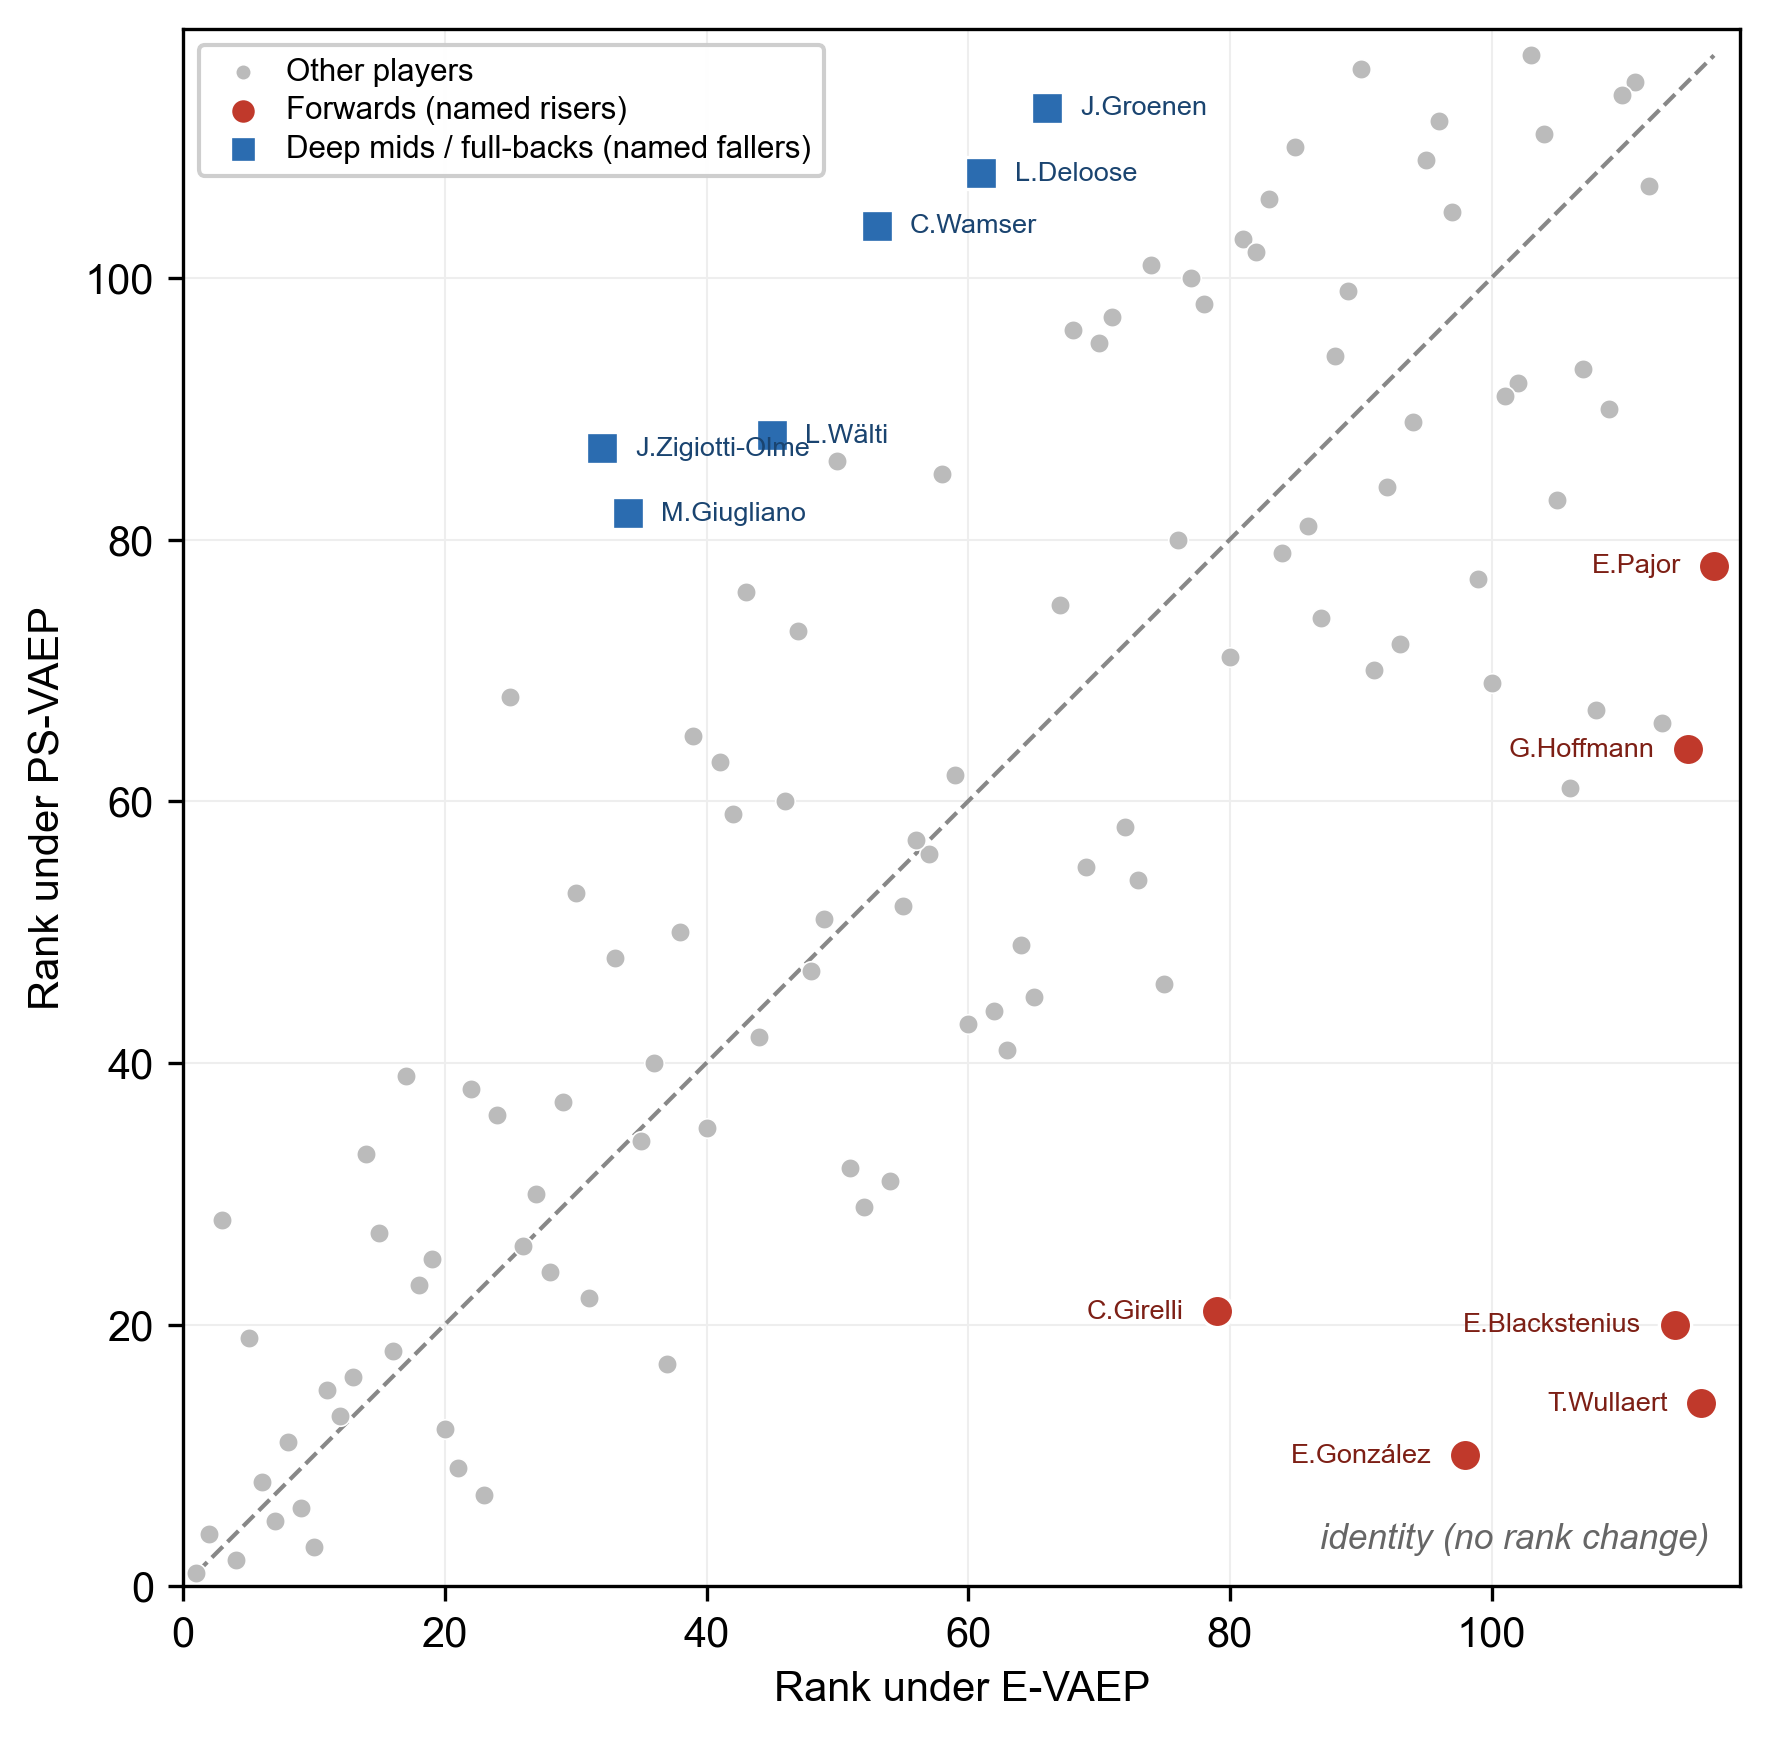
\includegraphics[width=\linewidth]{figures/figure_2.png}

\vspace{0.2em}
\footnotesize \textbf{(a)} Value per 90 under E-VAEP versus PS-VAEP
\end{minipage}
\hfill
\begin{minipage}[t]{0.40\textwidth}
\centering
\includegraphics[width=\linewidth]{figures/article_maanum}

\vspace{0.2em}
\footnotesize \textbf{(b)} Maanum take-on freeze frame.
\end{minipage}
\caption{Two views of PS-VAEP revaluation. Panel (a) shows player-level VAEP per 90 under both models: points above the diagonal indicate gains under PS-VAEP, and the shaded region contains players penalised by E-VAEP but rewarded by PS-VAEP. Panel (b) shows an action-level case in which dense local pressure leads PS-VAEP to assign a higher value than E-VAEP and P-VAEP.}
\label{fig:revaluation}
\end{figure}

Individual rank changes carry substantial uncertainty, as panel (a) of Fig.~\ref{fig:revaluation} shows: of the 117 qualifying players, only 25 have a rank change whose bootstrap interval excludes zero. Among those, the largest upward shifts are Severini ($+69$ ranks), Hoffmann ($+39$), Pajor ($+39$), Giuliani ($+35$), Tysiak ($+32$) and Naalsund ($+29$); the largest downward shifts are Groenen ($-51$), Deloose ($-48$), Zigiotti-Olme ($-32$) and Conca ($-21$). Both groups mix midfielders, forwards and defenders, so we do not claim that the redistribution follows positional lines: it is a broad reordering rather than a clean positional rotation.

We deliberately do not frame this redistribution as a correction. Reduced credit for progression through open space need not indicate over-valuation by the event-only model: such progression may be legitimately valuable, and in particular the space it exploits may have been created by preceding off-ball movement. Because our model values only on-ball actions, space creation is invisible to it, so the downward shift of deep-lying progressors is as consistent with a blind spot in PS-VAEP as with an error in E-VAEP. Distinguishing the two requires independent expert validation, which we have not performed.

\paragraph{Case study: a take-on under pressure.}
Panel (b) of Fig.~\ref{fig:revaluation} illustrates the action-level mechanism for a take-on by Frida Maanum against Iceland. The action occurs centrally in the penalty area, with four opponents within 5 m and four opponents between the ball and the goal. E-VAEP and P-VAEP assign negative values ($-0.196$ and $-0.200$), whereas PS-VAEP assigns a positive value ($+0.204$), which is consistent with the model treating ball retention under dense defensive pressure as valuable. This single action illustrates the mechanism that Section~\ref{sec:where} establishes systematically; on its own it would not support the interpretation.


\section{Discussion and Limitations}

The results separate two effects that are often conflated in action valuation. Tactical phase context improves probability estimation on the conceding head, and this is the only difference in the study that is separated from zero under both match-level resampling and seed variation. Freeze-frame spatial context does not improve aggregate prediction at this data scale --- and degrades it when added on top of phase --- yet it changes player valuation substantially. The $2 \times 2$ design shows the two layers to be substitutes on the predictive side, encoding overlapping information about how exposed a state is, while acting quite differently on the allocation side.

We should be equally clear about what we could not establish. The stratified analysis of Section~\ref{sec:where} does not identify which situations drive the reallocation: no stratum of density, pressure, zone, action type or outcome shows a robustly positive shift. An earlier version of this analysis did find one, and it did not survive retraining. We therefore report the reallocation as a phenomenon whose mechanism remains open.

This suggests that contextual valuation models should not be assessed only by ROC-AUC or log loss. A model can produce similar aggregate probability quality while reallocating credit across roles and tactical situations. In our setting, PS-VAEP is best interpreted as a revaluation model rather than a predictively superior model. Whether this redistribution is tactically preferable requires independent expert validation, which is left to future work.

Several limitations remain. The evaluation is restricted to one held-out women's tournament, and freeze-frame features observe only players visible in the broadcast frame rather than full tracking trajectories. The model values on-ball actions only, so off-ball runs that create space are not directly credited. The phase taxonomy is rule-based and may mislabel edge cases. Finally, the player-valuation redistribution has not yet been validated against independent expert assessment, and the freeze-frame coverage controls of Section~\ref{sec:visibility} bound rather than eliminate the possibility that part of the positional redistribution reflects broadcast framing.

The main conclusion is therefore not that more context always improves prediction, but that different context layers act on different aspects of valuation. The phase layer improves probability estimation; the spatial layer leaves it unchanged while reallocating credit across players and situations. That the P-VAEP versus PS-VAEP difference is not stable under resampling is not a negative result: it is the sharpest form of the prediction-versus-revaluation distinction we set out to draw.

Two findings that emerged from addressing the reviewers' concerns extend beyond that distinction. First, source-domain similarity in this setting is governed more by competition type than by gender: the men's club corpus is further from the women's international target ($\mathcal{A}$-distance $0.955$) than men's international football is ($0.713$), and at equal corpus size men's and women's training data are interchangeable. What a data-scarce target domain benefits from is more 360 data, whatever its provenance. Second, the spatial features are recoverable from event data well enough that a model built on predicted freeze frames matches one built on observed ones, which means the phase-and-space approach is not confined to the small set of competitions with 360 coverage. For women's football analytics, where event data is far more widely available than spatial data, that portability may matter more than the valuation results themselves.

\paragraph{Disclosure of Interests.}
The authors declare no competing interests.

% ---- Bibliography ----
\bibliographystyle{splncs04}
\bibliography{women_vaep_references}

\end{document}
